% Author: PokMan Ho pok.ho19@imperial.ac.uk
% Script: method.tex
% Desc: MRes thesis methods section
% Input: none
% Output: none
% Arguments: 0
% Date: Jan 2020

\documentclass[../thesis.tex]{subfiles} %% use packages & commands as this main file

\begin{document}
\section{Methodology}
%% 20200328
A minimal open microbial ecosystem was constructed with two players (phytoplankton and microbial detritivore) and three carbon pools (organic matter (C), phytoplankton biomass (P) and microbial biomass (B)).  Players were analogous to engines/machines, which took input materials and output processed matter(s).  This minimal system assumed the only resource was space for phytoplankton, while other commonly-known resources (such as light and nutrient) were unlimited.  Players and pools were inter-related as follow:

\begin{figure}[H]
    \centering
    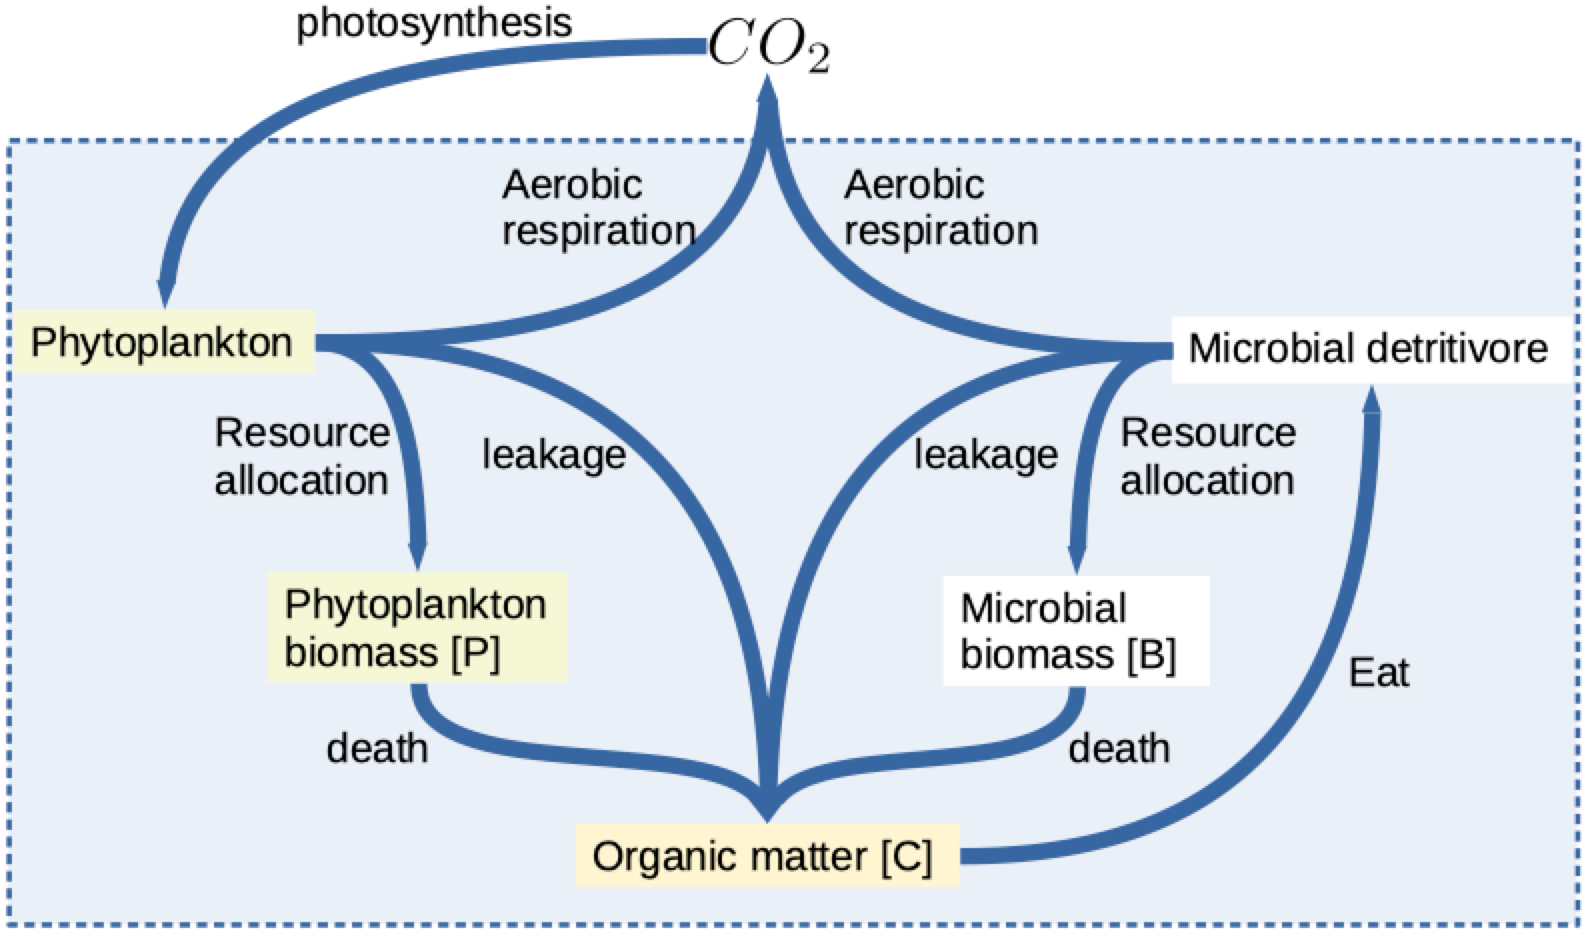
\includegraphics[width=\linewidth]{result/model.png}
    \caption{Classification of dominant interactions in this project.  The two players shared all interactions with respective carbon pools but one, which was the energy acquiring method.  This was due to all microbial cell membranes were not impermeable to carbon compounds as measured.(REF)  So apart from metabolism (i.e. aerobic respiration) and resource allocated to maintenance and population growth there was a portion of resource leakage.  Cellular life also were finite, hence death had to be considered as carbon pool transfer from biotic (i.e. biomass) to abiotic (i.e. organic matter) pools.  Due to the difference in energy acquiring strategies, phytoplanktons could extract carbon dioxide (CO$_2$) externally but detritivores could only take carbon from finite C pool.}
    \label{modelInWord}
\end{figure}

\end{document}
